%fich.tex
%%%%%%%%%%%%%%%%%%%%%%%%%%%%%%%%%%%%%%%%%%%%%%%%%%%%%%%%%%%%%%%%%%%%%%%%
% Fco. Javier Bóhorquez Ogalla
% Descripción del documento:
	
%%%%%%%%%%%%%%%%%%%%%%%%%%%%%%%%%%%%%%%%%%%%%%%%%%%%%%%%%%%%%%%%%%%%%%%%


%%%%%%%%%%%%%%%%%%%%%%%%%%%%%%%%%%%%%%%%%%%%%%%%%%%%%%%%%%%%%%%%%%%%%%%%
%Clase de documento
\documentclass[12pt, spanish]{article}
%%%%%%%%%%%%%%%%%%%%%%%%%%%%%%%%%%%%%%%%%%%%%%%%%%%%%%%%%%%%%%%%%%%%%%%%


%%%%%%%%%%%%%%%%%%%%%%%%%%%%%%%%%%%%%%%%%%%%%%%%%%%%%%%%%%%%%%%%%%%%%%%%	
%Paquetes de lenguaje:
%%%%%%%%%%%%%%%%%%%%%%%%%%%%%%%%%%%%%%%%%%%%%%%%%%%%%%%%%%%%%%%%%%%%%%%%
\usepackage[utf8]{inputenc}
\usepackage[spanish]{babel}
%\usepackage[spanish, activeacute] {babel}	
%\usepackage[spanish]{babel} 				
%\usepackage[latin1]{inputenc}
%%%%%%%%%%%%%%%%%%%%%%%%%%%%%%%%%%%%%%%%%%%%%%%%%%%%%%%%%%%%%%%%%%%%%%%%


%%%%%%%%%%%%%%%%%%%%%%%%%%%%%%%%%%%%%%%%%%%%%%%%%%%%%%%%%%%%%%%%%%%%%%%%
%Paquetes para encabezados y pie de páginas
%%%%%%%%%%%%%%%%%%%%%%%%%%%%%%%%%%%%%%%%%%%%%%%%%%%%%%%%%%%%%%%%%%%%%%%%
\usepackage{fancyhdr}
%%%%%%%%%
% \pagestyle{fancy} %Si se cambia el estilo de página, antes de empezar 
	%el documento. Esto hace que el emcabezado y pie de página se 
	%quede separado del texto por una línea
%%%%%%%%%	
% \fancyhead{} % Límpia el texto que se está usando como encabezado
%%%%%%%%%
% \fancyhead[OPCIONES]{Encabezado}
	% OPCIONES:
		% L texto a la izquierda
		% C texto centrado
		% R texto a la derecha
		% E página par
		% O pagina impar
	%Ejemplo: 
		% fancyhead [LE] {"Doc. Latex"} 
			% Establece como emcabezado de las páginas pares "Doc Latex"
			% con alineacion a la izquierda
%%%%%%%%%			
% \fancyfoot[OPCIONES]{Píe de pag.}
	% OPCIONES:
		% L C R E O
	%Ejemplo
		% \fancyfoot[LE,RO]{\thepage} 
			% Establece como píe de pág. el número de página. con 
			% alineación a la izq en paginas pares y a la derecha en
			% las impares
%%%%%%%%%			
% \renewcommand{\headrulewidth}{0.4pt}
% \renewcommand{\footrulewidth}{0.4pt}
	% Fija el grosor de la la linea que separa el emcabezado y pie de pág
%%%%%%%%%
% Otros comandos:
%\lhead{}
%\chead{}
%\rhead{}
%\lfoot{}
%\cfoot{}
%%%%%%%%%%%%%%%%%%%%%%%%%%%%%%%%%%%%%%%%%%%%%%%%%%%%%%%%%%%%%%%%%%%%%%%%


%%%%%%%%%%%%%%%%%%%%%%%%%%%%%%%%%%%%%%%%%%%%%%%%%%%%%%%%%%%%%%%%%%%%%%%%
% Paquetes para tamaños y distancias
%%%%%%%%%%%%%%%%%%%%%%%%%%%%%%%%%%%%%%%%%%%%%%%%%%%%%%%%%%%%%%%%%%%%%%%%
\usepackage{anysize} 
%%%%%%%%%%%
% \marginsize{3cm}{2cm}{2cm}{2cm}
	% Controla los márgenes {izquierda}{derecha}{arriba}{abajo}. 
%%%%%%%%%%%%%%%%%%%%%%%%%%%%%%%%%%%%%%%%%%%%%%%%%%%%%%%%%%%%%%%%%%%%%%%%


%%%%%%%%%%%%%%%%%%%%%%%%%%%%%%%%%%%%%%%%%%%%%%%%%%%%%%%%%%%%%%%%%%%%%%%%
%Paquetes de carácteres especiales:
%%%%%%%%%%%%%%%%%%%%%%%%%%%%%%%%%%%%%%%%%%%%%%%%%%%%%%%%%%%%%%%%%%%%%%%%
\usepackage{dsfont}	
%Para representar conjuntos matematicos comunes: Z, N, R...
	% mathds{R}, mathds{N},...
%%%%%%%%%%%%%%%%%%%%%%%%%%%%%%%%%%%%%%%%%%%%%%%%%%%%%%%%%%%%%%%%%%%%%%%%

%%%%%%%%%%%%%%%%%%%%%%%%%%%%%%%%%%%%%%%%%%%%%%%%%%%%%%%%%%%%%%%%%%%%%%%%
%Paquetes para insertar gráficos
%%%%%%%%%%%%%%%%%%%%%%%%%%%%%%%%%%%%%%%%%%%%%%%%%%%%%%%%%%%%%%%%%%%%%%%%
\usepackage[dvips]{graphicx}
\DeclareGraphicsExtensions{.pdf,.png,.jpg} %solo para PDFLaTeX
%%%%%%%%%%%%%%%%%%%%%%%%%%%%%%%%%%%%%%%%%%%%%%%%%%%%%%%%%%%%%%%%%%%%%%%%

%%%%%%%%%%%%%%%%%%%%%%%%%%%%%%%%%%%%%%%%%%%%%%%%%%%%%%%%%%%%%%%%%%%%%%%%
%Paquetes de color:
%%%%%%%%%%%%%%%%%%%%%%%%%%%%%%%%%%%%%%%%%%%%%%%%%%%%%%%%%%%%%%%%%%%%%%%%
\usepackage{color}
%%%%%%%%%%%%%%%%%%%%%%%%%%%%%%%%%%%%%%%%%%%%%%%%%%%%%%%%%%%%%%%%%%%%%%%%
%Definición de colores:
\definecolor{gray97}{gray}{.97}
\definecolor{gray75}{gray}{.75}
\definecolor{gray45}{gray}{.45}
%%%%%%%%%%%%%%%%%%%%%%%%%%%%%%%%%%%%%%%%%%%%%%%%%%%%%%%%%%%%%%%%%%%%%%%%


%%%%%%%%%%%%%%%%%%%%%%%%%%%%%%%%%%%%%%%%%%%%%%%%%%%%%%%%%%%%%%%%%%%%%%%%
%Paquete de listado de código:
%%%%%%%%%%%%%%%%%%%%%%%%%%%%%%%%%%%%%%%%%%%%%%%%%%%%%%%%%%%%%%%%%%%%%%%%
\usepackage{listings}
%%%%%%%%%%%%%%%%%%%%%%%%%%%%%%%%%%%%%%%%%%%%%%%%%%%%%%%%%%%%%%%%%%%%%%%%
%Configuración del listado:
\lstset { 
	frame=Ltb,
     framerule=0pt,
     aboveskip=0.2cm,
     framextopmargin=0.3pt,
     framexbottommargin=0.2pt,
     framexleftmargin=0.3cm,
     framesep=0pt,
     rulesep=.1pt,
     tabsize=2,
     backgroundcolor=\color{gray97},
     rulesepcolor=\color{black},
     %
     stringstyle=\ttfamily,
     showstringspaces = false,
     basicstyle=\scriptsize\ttfamily,
     commentstyle=\color{gray45},
     keywordstyle=\bfseries,
   	%
     numbers=left,
     numbersep=1pt,
     numberstyle=\tiny,
     numberfirstline = false,
     breaklines=true,
}
%%%%%%%%%%%%%%%%%%%%%%%%%%%%%%%%%%%%%%%%%%%%%%%%%%%%%%%%%%%%%%%%%%%%%%%%


%%%%%%%%%%%%%%%%%%%%%%%%%%%%%%%%%%%%%%%%%%%%%%%%%%%%%%%%%%%%%%%%%%%%%%%%
%Indexado. Índice alfabeticos
\usepackage{makeidx}
\makeindex %para habilitar indices
%%%%%%%%%%%%%%%%%%%%%%%%%%%%%%%%%%%%%%%%%%%%%%%%%%%%%%%%%%%%%%%%%%%%%%%%
%Forma de uso:
% \index{clave} %Para crear un indice de materia
% Supongase que queremos meter en el indice alfabetico referencias a 
% las paginas donde se hace referencia a la clave Producto escalar
% en tal caso en cada una de las páginas pondremos \index{Producto escalar}
% \printindex %Para imprimir el índice alfabetico

% Es necesario una doble compilación del documento. La primera genera un 
% fichero.idx el cual tendremos que procesar con la aplicación makeindex
%tras procesarlo se creará un fichero.ind que contendra el código Latex 
% que se inserta en el documento original. 
% Tras la segunda compilación del documento original se sustituira el
% comando \printindex por el contenido del fichero.ind 

%Podemos cambiar el formato de la clave:
%Ejemplo     				&    	Entrada 		&	Comentario
%\index{hola}				&         hola, 1   	&	Entrada simple
%\index{hola!Pedro}			&		 Pedro, 3 	&	Subentrada bajo ‘hola’
%\index{Juan@\textsl{Juan}}  	&		Juan, 2    	&	Entrada con diseño                        
%\index{Pepa@\textbf{Pepa}}	&		Pepa, 7    	&	Igual que antes
%\index{Loli|textbf}		&		Loli, 3    	&	No de página con diseño                     
%\index{Soraya|textit}		&		Soraya, 5  	&	Igual que antes
%%%%%%%%%%%%%%%%%%%%%%%%%%%%%%%%%%%%%%%%%%%%%%%%%%%%%%%%%%%%%%%%%%%%%%%%


%%%%%%%%%%%%%%%%%%%%%%%%%%%%%%%%%%%%%%%%%%%%%%%%%%%%%%%%%%%%%%%%%%%%%%%%


%%%%%%%%%%%%%%%%%%%%%%%%%%%%%%%%%%%%%%%%%%%%%%%%%%%%%%%%%%%%%%%%%%%%%%%%
%Estilo de página
%%%%%%%%%%%%%%%%%%%%%%%%%%%%%%%%%%%%%%%%%%%%%%%%%%%%%%%%%%%%%%%%%%%%%%%%
%\textwidth 6.75in								  %ancho de texto
%\oddsidemargin -0.2in							%margen izquierdo 
\parskip 0.2in									%espacio parrafos
%%%%%%%%%%%%%%%%%%%%%%%%%%%%%%%%%%%%%%%%%%%%%%%%%%%%%%%%%%%%%%%%%%%%%%%%
\newenvironment{changemargin}[2]{%
\begin{list}{}{%
\setlength{\topsep}{300pt}%
\setlength{\leftmargin}{#1}%
\setlength{\rightmargin}{#2}%
\setlength{\listparindent}{\parindent}%
\setlength{\itemindent}{\parindent}%
\setlength{\parsep}{\parskip}%
}%
\item[]}{\end{list}}
%%%%%%%%%%%%%%%%%%%%%%%%%%%%%%%%%%%%%%%%%%%%%%%%%%%%%%%%%%%%%%%%%%%%%%%%
\usepackage{float}
\restylefloat{table}
\usepackage{placeins}
\usepackage{framed}
\usepackage{epsf}
%%%%%%%%%%%%%%%%%%%%%%%%%%%%%%%%%%%%%%%%%%%%%%%%%%%%%%%%%%%%%%%%%%%%%%%%

\usepackage{titlesec}

\setcounter{secnumdepth}{4}

\titleformat{\paragraph}
{\normalfont\normalsize\bfseries}{\theparagraph}{1em}{}
\titlespacing*{\paragraph}
{0pt}{3.25ex plus 1ex minus .2ex}{1.5ex plus .2ex}


%%%%%%%%%%%%%%%%%%%%%%%%%%%%%%%%%%%%%%%%%%%%%%%%%%%%%%%%%%%%%%%%%%%%%%%%	
%datos del documento
\author{modelo de comportamineto básico \\\\\ Fco. Javier Bohórquez Ogalla}						%autor
\date{}														%fecha

\title{ 
\begin{center}

\includegraphics[scale=0.5]{logo-doc.png}
\end{center} 
}
%%%%%%%%%%%%%%%%%%%%%%%%%%%%%%%%%%%%%%%%%%%%%%%%%%%%%%%%%%%%%%%%%%%%%%%%

%%%%%%%%%%%%%%%%%%%%%%%%%%%%%%%%%%%%%%%%%%%%%%%%%%%%%%%%%%%%%%%%%%%%%%%%
%Documento:
%%%%%%%%%%%%%%%%%%%%%%%%%%%%%%%%%%%%%%%%%%%%%%%%%%%%%%%%%%%%%%%%%%%%%%%%
\begin{document}

\maketitle
\pagebreak
\tableofcontents
\pagebreak
% ======================================================================
\section{Diseño de componentes}
El presente documento constituye el modelo de comportamiento básico.
Este detalla cómo los distintos objetos interaccionan y se comunican entre sí para
analizar la entrada del usuario, correspondiente el código fuente, e interpretarlo
para su ejecución.

Se presenta un diagrama de secuencia para la operación interpretación
de un código fuente. Luego se presenta diagramas de comunicación correspondientes
a algunas sentencias escritas en el lenguaje.


% ======================================================================
\subsection{Interpretar código fuente}
Para la interpretación de código fuente el sistema crea los objetos 
encargados del análisis léxico y sintáctico del mismo. El objeto principal
del sistema se encarga de crear e inicializar el analizador sintáctico (parser) a
partir del código fuente, a su vez este crea el analizador léxico (scanner)
que crea una estructura correspondiente al código fuente que será interpretado.

El sistema envía un mensaje para que el parser analice el código fuente.
El analizador sintáctico define una serie de reglas gramaticales e irá comprobando que 
el código fuente cumple estas reglas a la vez que las utiliza para crear un árbol de derivación 
denominado árbol sintáctico. Para ello hace uso de una serie de tokens que irá solicitando 
al analizador léxico. Este último obtendrá los tokens a partir del código fuente, mediante 
una serie de reglas léxicas formadas a partir de lenguajes regulares. Por cada regla 
gramatical que se cumpla en el parser, este habrá obtenido del scanner tantos tokens como 
componentes léxicos sean necesarios para cumplir la regla. Además por cada regla gramatical se
construirá un nodo ejecutable formado a partir del valor asociado a una serie de tokens, o 
a partir de otros nodos ejecutables construidos por reglas de mayor prioridad y creados en 
anteriores interacciones. Esto formará un árbol sintáctico formado por nodos ejecutables que 
contienen la semántica que encierran las construcciones del código fuente.

A partir del nodo raíz del árbol de nodos ejecutables comienza un recorrido en profundidad del
árbol que conllevará la ejecución del código fuente, produciéndose así el resultado semántico 
esperado.

En el caso de que no se de una regla gramatical que se corresponda con el código analizado se 
producirá un error sintáctico. Por otro lado, en el caso de que alguna cadena contenida
en el código fuente no se corresponda con los lenguajes regulares que define el scanner
se producirá un error léxico.


\begin{center}
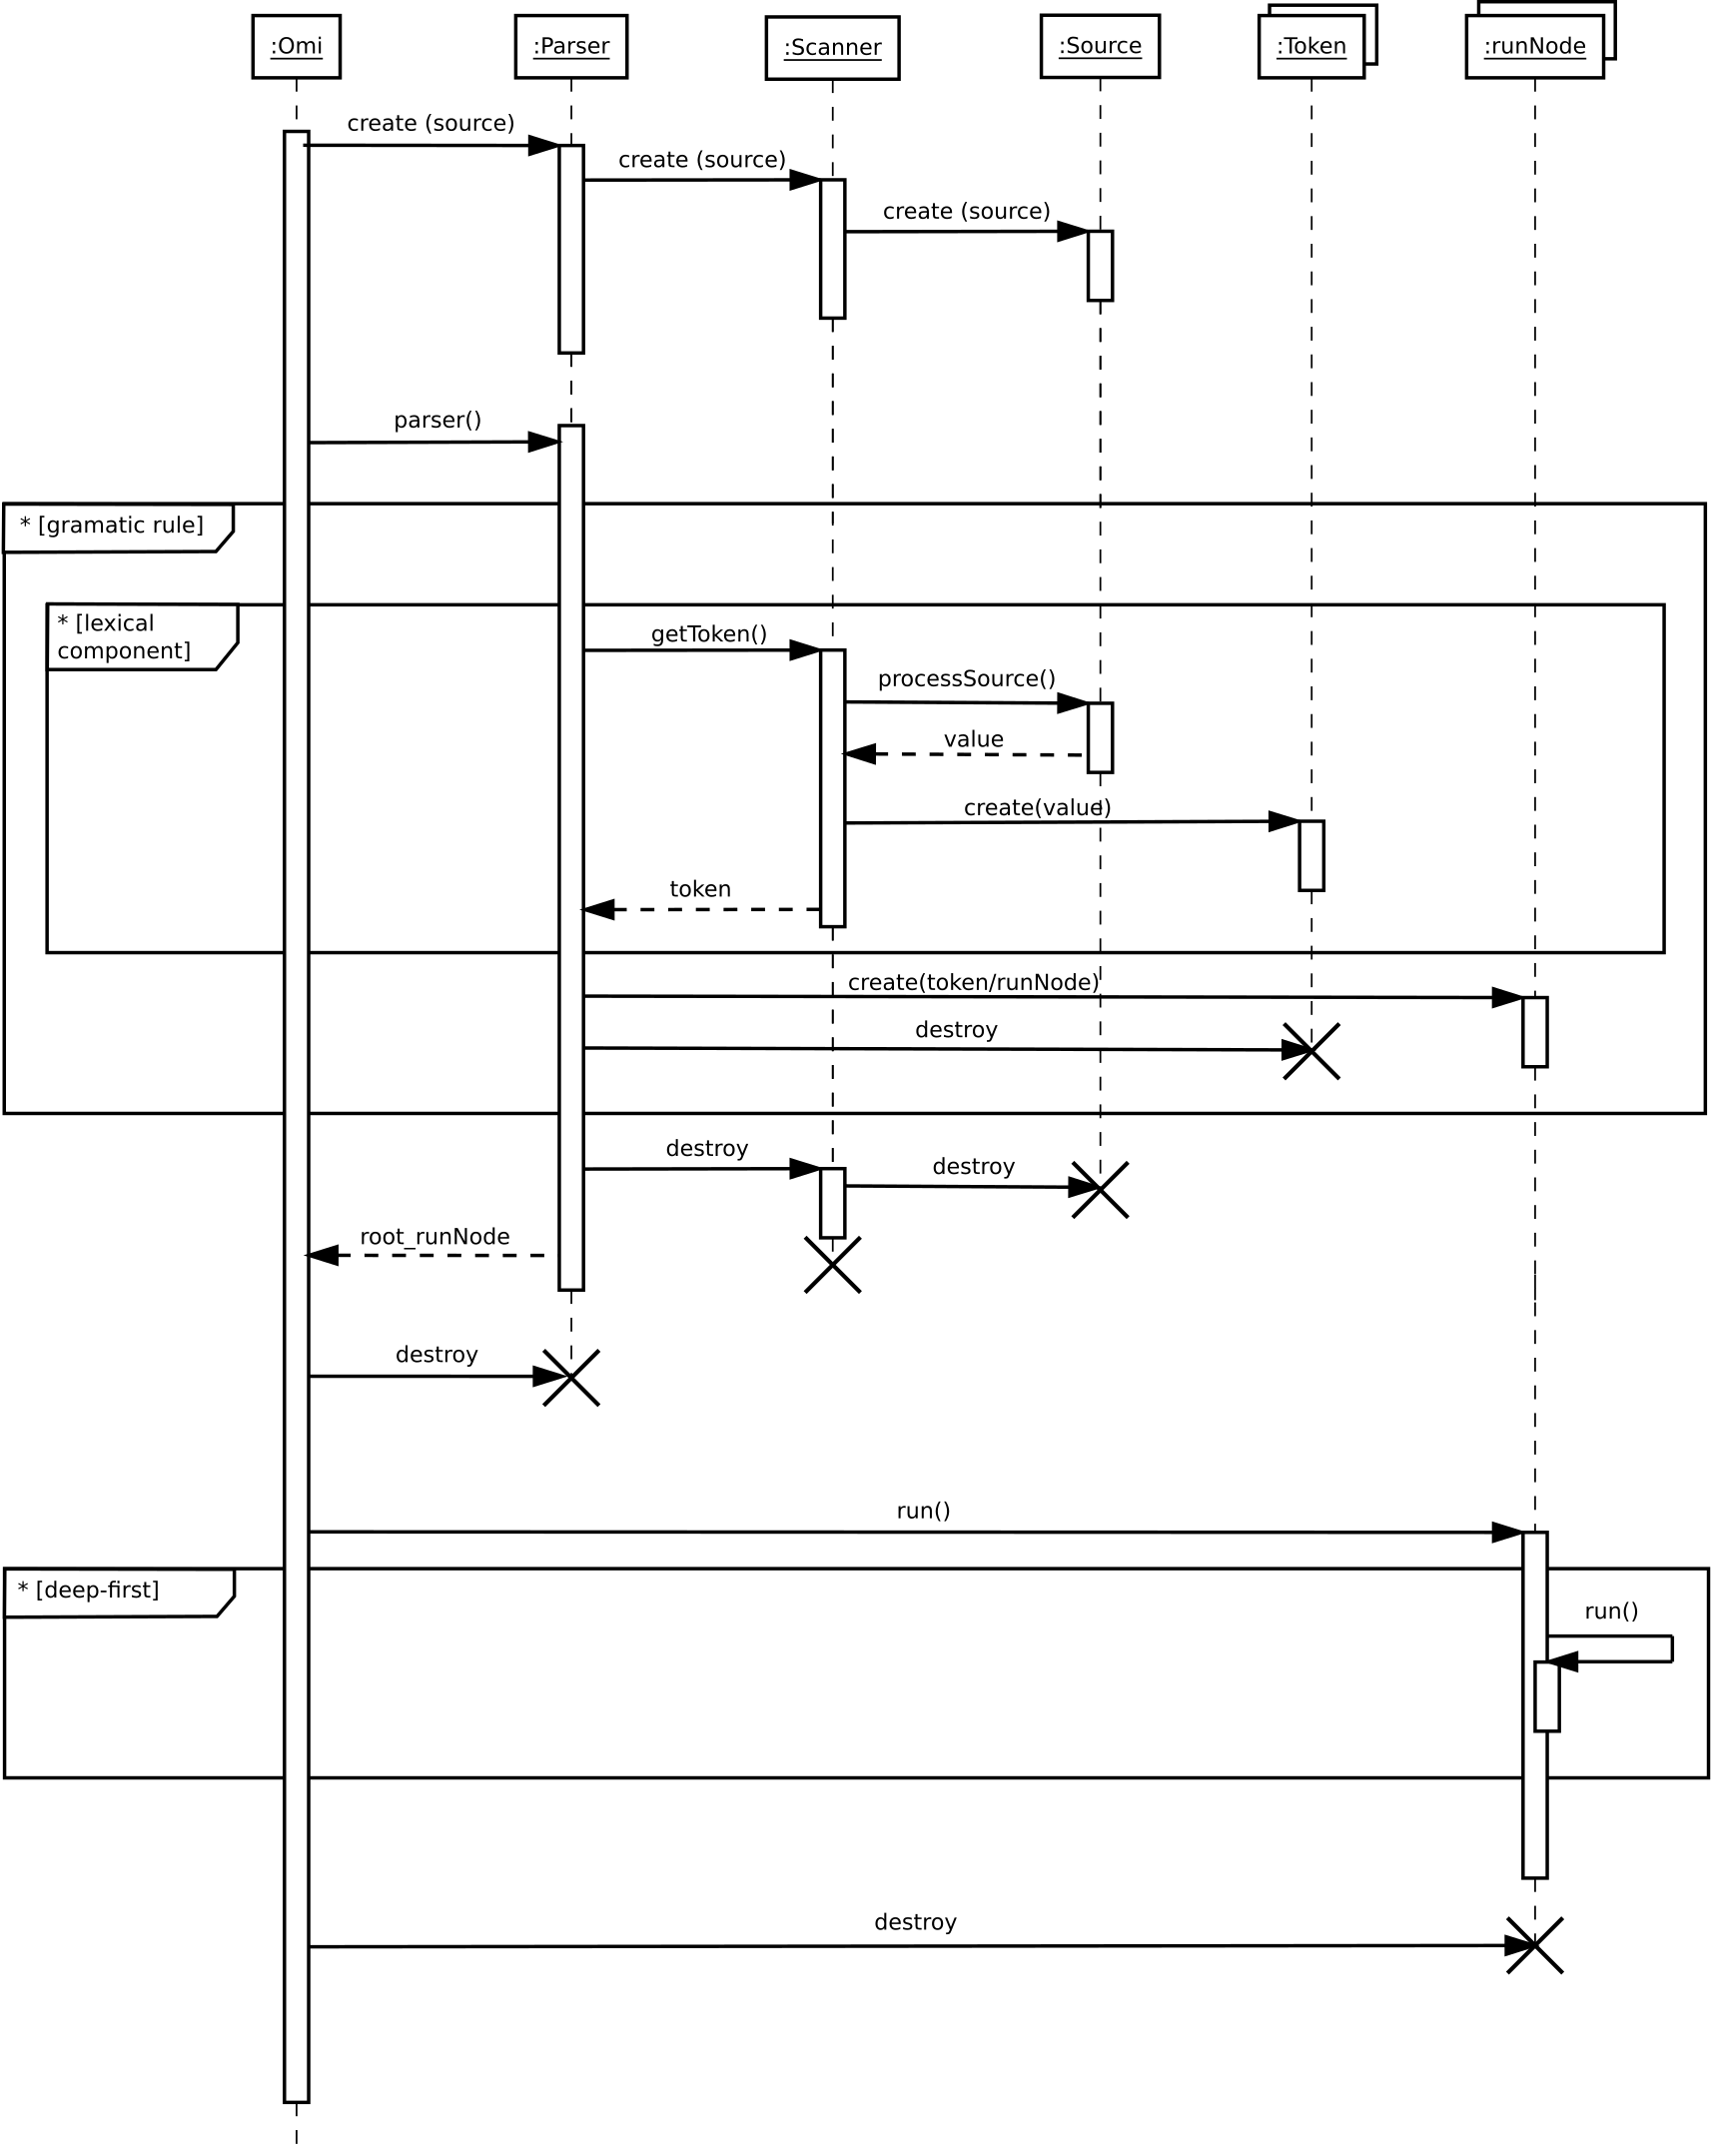
\includegraphics[scale=0.32]{interaction.png} \\
\end{center}

\subsection{Sentencias}
\subsubsection {Sentencia de control condicional }
\begin{center}
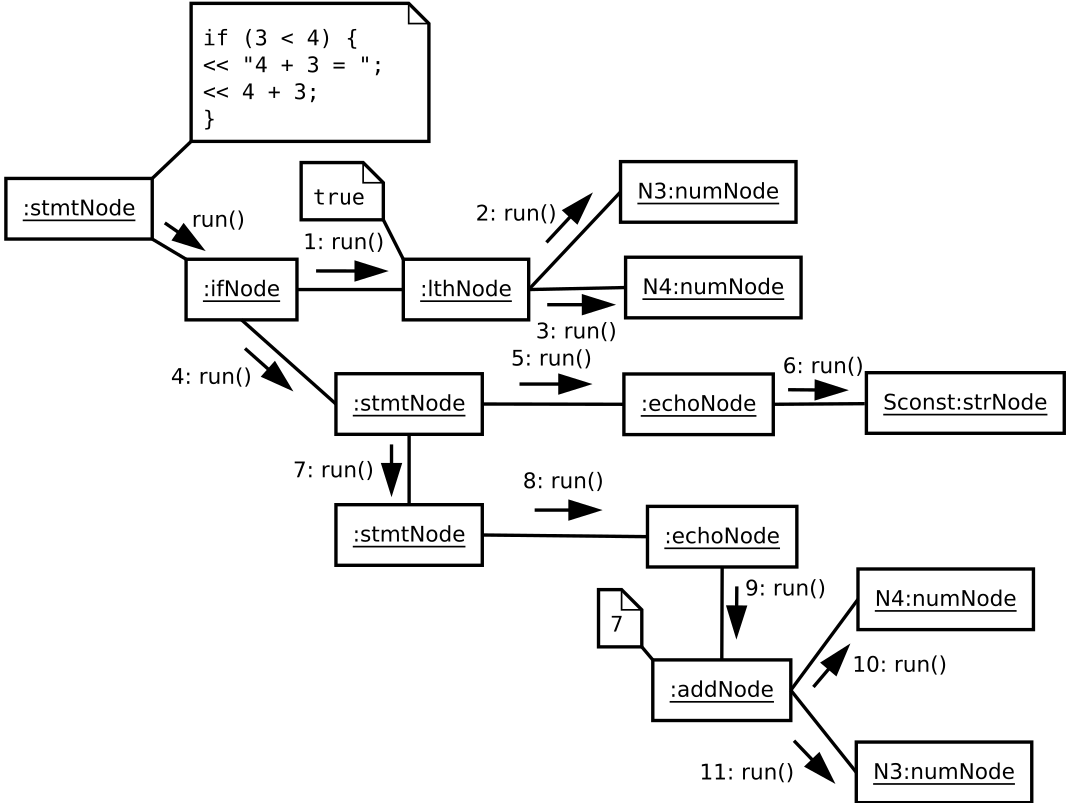
\includegraphics[scale=0.38]{if.png} \\
\end{center}

\subsubsection {Operaciones aritméticas }
\begin{center}
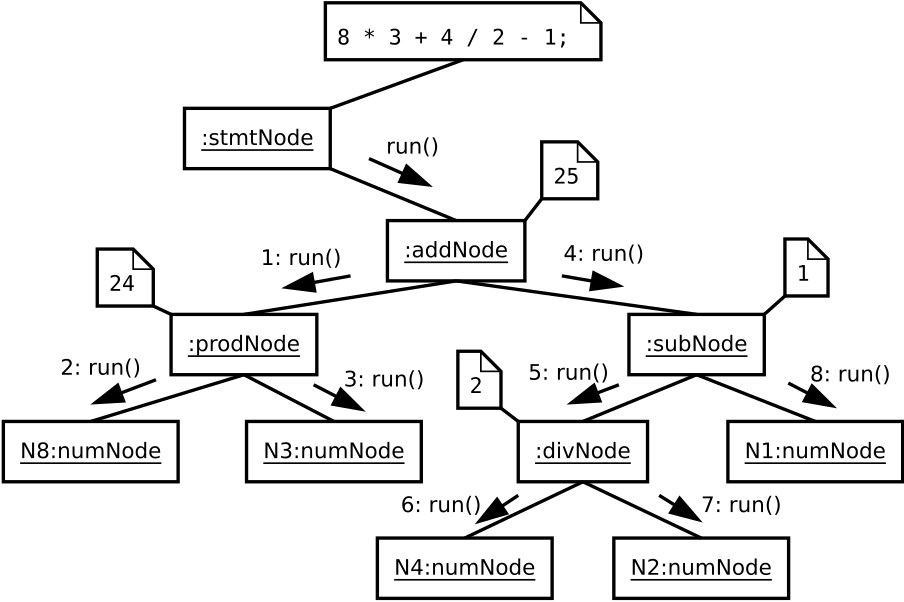
\includegraphics[scale=0.38]{arith.png} \\
\end{center}

\subsubsection {Asignaciones }
\begin{center}
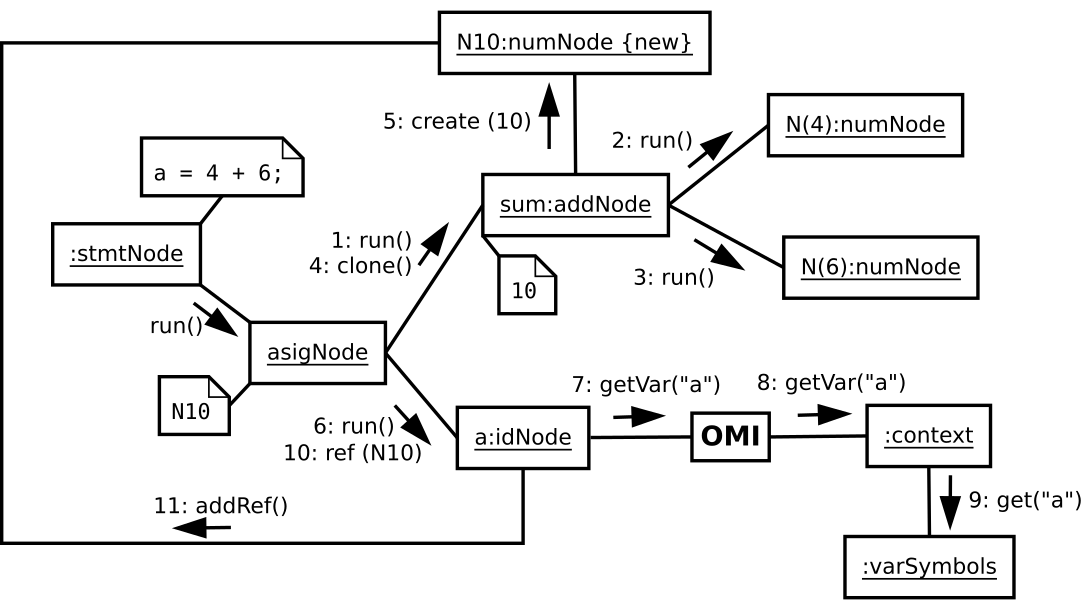
\includegraphics[scale=0.38]{asig.png} \\
\end{center}

\begin{center}
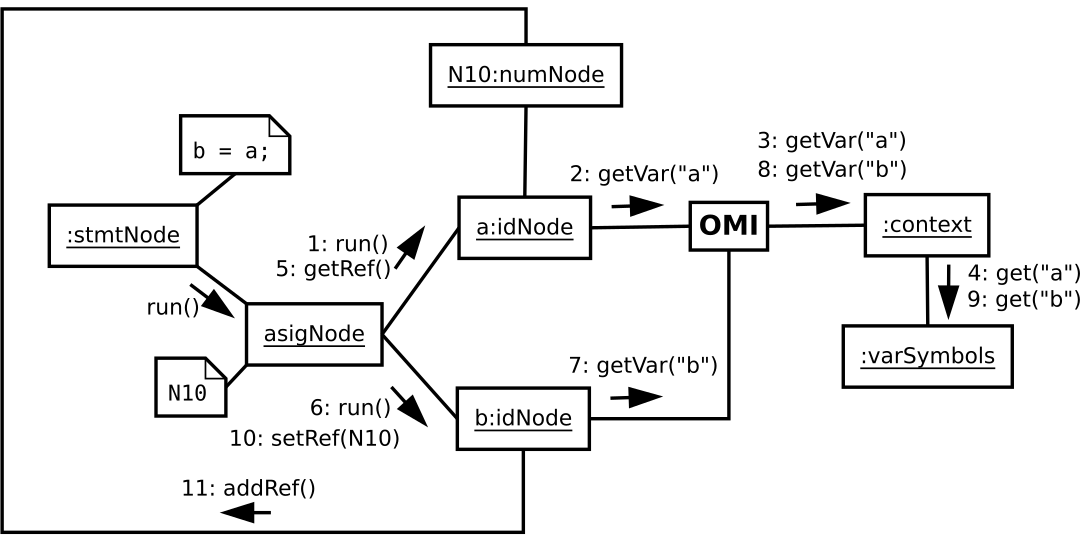
\includegraphics[scale=0.38]{asig2.png} \\
\end{center}

\begin{center}
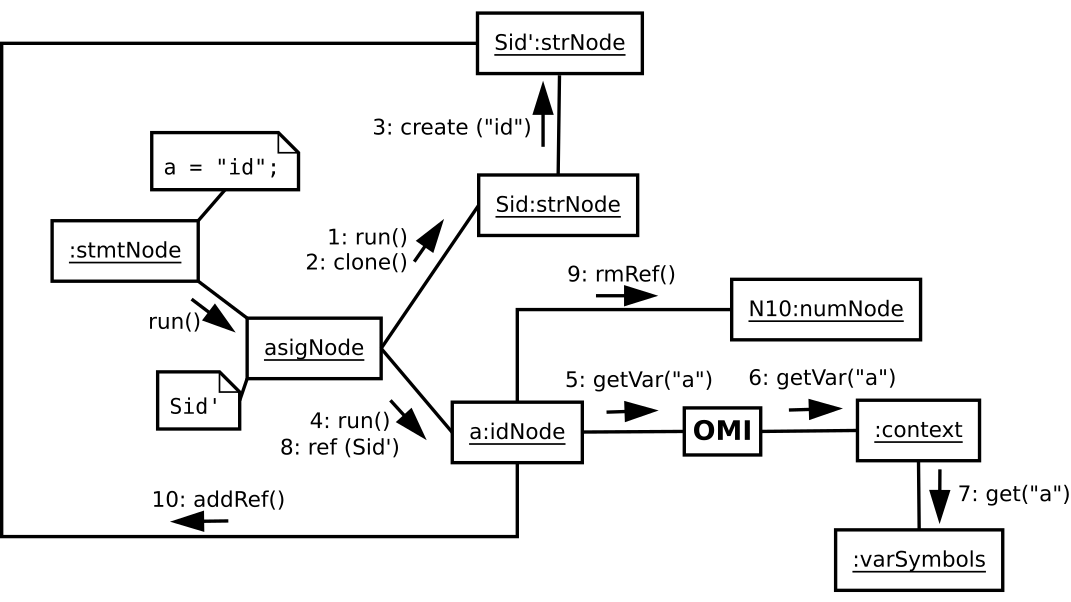
\includegraphics[scale=0.38]{asig3.png} \\
\end{center}

% ----------------------------------------------------------------------

\end{document}
%%%%%%%%%%%%%%%%%%%%%%%%%%%%%%%%%%%%%%%%%%%%%%%%%%%%%%%%%%%%%%%%%%%%%%%%
%Fco. Javier Bohórquez Ogalla
